\documentclass[11pt,a4paper,oneside]{report}
\usepackage[utf8]{inputenc}
\usepackage[T1]{fontenc}
\usepackage{lmodern}
\usepackage{microtype}
\usepackage[a4paper,margin=1in]{geometry}
\usepackage{amsmath,amssymb}
\usepackage{booktabs,array,tabularx,longtable}
\usepackage{enumitem}
\usepackage{graphicx}
\usepackage{pdfpages}
\usepackage{xcolor}
\definecolor{accent}{HTML}{1F3A5F}
\usepackage[colorlinks=true,linkcolor=accent,citecolor=accent,urlcolor=accent]{hyperref}
\usepackage{caption}
\captionsetup{font=small,labelfont=bf}
\usepackage{setspace}
\setstretch{1.2}
\setlist{itemsep=2pt,topsep=4pt}
\graphicspath{{../reports/figs/}}
\newcolumntype{L}{>{\raggedright\arraybackslash}X}
\newcommand{\bp}{\,bp}

\begin{document}

\begin{titlepage}
\centering
\vspace*{3cm}
{\LARGE\bfseries\color{accent} Limits to Arbitrage in the Indian Equity Market\par}
\vspace{1.2cm}
{\large Bachelor's Thesis (EC 495 and EC 497)\par}
\vspace{0.6cm}
{\large Prince Kumar (23B3032)\par}
{BS Economics, Indian Institute of Technology Bombay\par}
\vspace{0.6cm}
{Guide: Prof.\ Aditi Chaubal\par}
\vfill
{Draft, November 2026\par}
\end{titlepage}

\begin{abstract}
In theory, a share and a future on that share should be priced consistently, and arbitrage should close any gap. In
practice costs, short-sale constraints, limited capital and position limits allow gaps to persist. I study how strongly
these limits bind in Indian equities, where most of them change on known dates. A model of constrained arbitrage, in
which India's F\&O ban is a rule that lets every participant only reduce positions, gives predictions and the results
that would contradict them; the tests were written down and frozen before any outcome was related to any treatment. The
data are built from public exchange files for 2015 to 2026. Bans bind hard on trading: futures volume falls by about two
log points, and when the rule is enforced on intraday positions every futures trade closes positions. Correction of the
futures-cash basis does not become one-sided in the way the model predicts: rich futures revert faster in a ban, mostly at
the start of a spell. The basis falls by about six basis points when a ban begins, more when open interest was building
fast, and there is no bunching of utilisation below the trigger. The basis follows a wide, asymmetric band of about $-35$
to $+24$ basis points around each stock's median, and the full cost of a new cash-and-carry position lies in its outer
tail. Entry into the F\&O segment speeds up the response of prices to market news but does not weaken drift after bad
news. A constraint index built only from frictions predicts slower price adjustment and larger drift after bad, but not
good, news across the whole market.
\end{abstract}

\tableofcontents

\chapter{Introduction}\label{ch:intro}

\section{The question}
When two ways of holding the same risk trade at different prices, an arbitrageur can buy the cheap one, sell the dear one
and wait for the prices to meet. If arbitrage were free and unlimited, such gaps would never be large or long-lived.
Shleifer and Vishny (1997) and Gromb and Vayanos (2010) explain why it is neither: arbitrage needs capital, it carries
risk while the gap persists, it costs money to trade, and it often needs a short position that may be costly or not
allowed. Each of these limits lets prices drift away from each other.

This thesis asks how strongly these limits bind in the Indian equity market, which of them matter, and how much
mispricing they explain. India is a good place to ask. Almost every limit changes on known dates: the securities
transaction tax (STT) on futures was raised three times between 2023 and 2026; only stocks in the futures and options
(F\&O) segment can be sold short or shorted through stock futures, and stocks enter and leave that segment every few
months; the assets of arbitrage mutual funds grew several times after a change in the taxation of debt funds in 2023; and
position limits are set by formula and were changed in October 2025.

India also has an unusual rule. When market-wide open interest in a stock's derivatives exceeds 95\% of its market-wide
position limit (MWPL), the stock enters an \emph{F\&O ban}: every participant, not only arbitrageurs, may only trade to
reduce positions until open interest falls to 80\%. Between 2015 and October 2026 this happened 1,788 times to 141 stocks.
To my knowledge no study has estimated its effects. The ban is the sharpest lens on one limit, but it is one lens among
several; the thesis studies the limits side by side.

\section{Approach}
The work followed a fixed order, designed to prevent fitting the theory and the data to each other.
\begin{enumerate}
\item \emph{Theory first.} One model covers all the limits; each enters as a parameter. The ban is modelled as the rule
actually works. Every hypothesis is derived from the model with the result that would contradict it (Chapter~\ref{ch:theory}).
\item \emph{A frozen test plan.} Samples, variables, specifications and falsifiers were written down and frozen with a
time-stamped record before any outcome was related to any treatment. Every detail the plan left open was fixed in a dated
log before the test that needed it was run (Appendix~\ref{app:plan}).
\item \emph{Data from primary sources.} All data come from public exchange archives and are built with scripts that check
every step against the exchange's own rules (Chapter~\ref{ch:data}).
\item \emph{Estimators tested on simulated data} from the model before use.
\item \emph{All results reported,} including those that contradict the model.
\end{enumerate}

\section{Main findings}
\begin{enumerate}
\item \textbf{Bans bind on trading.} In a ban, futures trading falls by about two log points and the delivery share of cash
trading rises. When the rule was enforced on peak intraday positions (March 2020 to September 2025), the change in open
interest equals minus the volume: every futures trade closed a long and a short. Under end-of-day enforcement before March
2020 this identity did not hold.
\item \textbf{Correction is not one-sided as predicted.} The model predicts that rich futures stop being corrected in a ban
because nobody may open new cash-and-carry positions. The data show the opposite: rich futures revert faster in a ban, and
cheap futures more slowly. The effect is concentrated in the first days of a spell and survives a correction for noise in
daily prices.
\item \textbf{The basis falls when a ban starts.} Against stocks that came close to the trigger but did not cross it, the
basis is about 6 basis points (bp) lower in the first days of a ban, more when open interest had been building fast, and
it returns to its earlier level after about a week. Utilisation does not bunch below the trigger, and as utilisation rises
the basis is more often rich.
\item \textbf{Costs, capital and the band.} The basis follows a wide, asymmetric band, about $-35$ to $+24$\bp\ around each
stock's median. The upper part of the distribution rose around the 2024 and 2026 STT increases, but by more than the cost
changes and mostly as a common shift. A new cash-and-carry round trip costs 27 to 31\bp, which places it in the outer tail
of the basis; rolling an existing position costs 4 to 8\bp. Inflows into arbitrage funds are followed by a lower upper
tail, but the evidence is weak.
\item \textbf{Short-sale access and the cross-section.} After a stock enters the F\&O segment its price responds faster to
market-wide news; drift after bad news does not weaken. A constraint index built only from frictions, for every listed
stock, predicts slower price adjustment, also after controlling for size; its link with drift after bad news is a size
effect.
\end{enumerate}

\section{Contribution}
The thesis studies the F\&O ban for the first time; models it as a reduce-only rule for every participant and shows that
this makes correction one-sided in theory and the level effect ambiguous in sign; shows that changes in the position limit
cannot serve as an instrument for ban status; estimates the no-arbitrage band of Indian stock futures over a long daily
sample with threshold and smooth-transition models; and publishes a constraint index for all Indian stocks. The closest
earlier work on Indian stock futures estimates bands from intraday data over short samples without the ban (Aggarwal,
2015; Shankar, Sankar and Kiran Kumar, 2019); Saurav, Srivastava and Agarwalla (2026) study the basis around earnings
announcements and short-sale constraints.

\section{Outline}
Chapter~\ref{ch:inst} describes the Indian rules. Chapter~\ref{ch:theory} presents the model. Chapter~\ref{ch:data}
describes the data, the measures and the constraint index. Chapter~\ref{ch:band} estimates the band and relates it to
costs, capital and position limits. Chapter~\ref{ch:ban} studies the ban. Chapter~\ref{ch:elig} studies entry into and exit
from the F\&O segment and the cross-section of stocks. Chapter~\ref{ch:concl} concludes and discusses policy.

\chapter{Institutional setting}\label{ch:inst}
\chapterlead{The Indian rules that shape each limit to arbitrage: who may sell short, which stocks have derivatives, how
the position limit and the ban work and how they were enforced, what trading costs, and where arbitrage capital comes
from. Figure~\ref{fig:timeline} places the dated changes on one time line.}

\begin{figure}[t]
\caption[The dated changes to the limits, 2015 to 2026]{Almost every limit to arbitrage changed on a known date during the sample}\label{fig:timeline}
\exsub{Futures STT, enforcement of the ban, the position-limit rule and arbitrage capital, 2015 to 2026}
\centering\includegraphics[width=\linewidth]{fig_timeline}
\exsource{Source: SEBI circulars and press releases, NSE circulars (listed in the references).}
\end{figure}

\section{Short selling and securities lending}
Under SEBI's short-selling framework (restated in a circular of 5 January 2024, in line with the 2007 framework), all
classes of investors may sell short, but naked short selling is prohibited: every short sale must be delivered at
settlement. Institutional investors may not day trade. Securities traded in the F\&O segment are eligible for short
selling. An overnight short in the cash market therefore needs borrowed stock, which comes from the securities lending
and borrowing (SLB) segment. SLB covers F\&O stocks and, since July 2013, other liquid stocks that meet the exchanges'
criteria, but trading in it is thin: on a typical day a few dozen stocks are lent. In practice the overnight short in an
Indian stock is a short single-stock future (or an options position), and this exists only for F\&O stocks. Stock
derivatives have been physically settled since the October 2019 expiry.

\section{The F\&O segment}
A stock enters the F\&O segment when it meets SEBI's eligibility criteria (market capitalisation, traded value, order size,
MWPL and delivery value; the criteria were tightened in 2018 and again on 30 August 2024) and leaves it after failing them.
From 2015 to October 2026 there were 239 entries and 171 exits, 162 of them eligibility exits after which the stock kept
trading in the cash market. Entry gives a stock futures and options and formal short-selling eligibility at once, and
exit removes them.

\section{The market-wide position limit and the ban}
\begin{table}[t]
\caption[Position-limit rules over the sample]{The limit was cut and open interest redefined in October 2025}\label{tab:mwpl}
\exsub{Market-wide position limit (MWPL) and the open interest tested against it}
\small\begin{tabularx}{\textwidth}{@{}K{3.2cm}LL@{}}
\toprule
\thd{Period} & \thd{MWPL} & \thd{Open interest tested} \\
\midrule
To 30 Sep 2025 & 20\% of shares held by non-promoters (free float) & Gross open interest, futures and options \\ \rowrule
20 Mar to 26 Nov 2020 & Halved for volatile or heavily used stocks (61 stocks) & Gross open interest \\ \rowrule
From 1 Oct 2025 & Lower of 15\% of free float and 65 times average daily delivery (in shares), floor 10\% of free float; recomputed quarterly & Futures-equivalent (delta-adjusted) open interest \\
\bottomrule
\end{tabularx}
\exsource{Source: SEBI circulars of 22 September 2006 and 29 May 2025; SEBI press release 18/2020; NSE Clearing circular 119/2025.}
\end{table}

A stock enters the ban when market-wide open interest exceeds 95\% of its MWPL at the end of a day, from the next day, and
leaves it when open interest falls to 80\%. During the ban every participant may only reduce positions, in all expiries
and in both futures and options; rolling a position into the next expiry is not permitted. How the rule was enforced
changed twice, and the changes matter for the results:
\begin{itemize}
\item \emph{Until 22 March 2020}, violations were judged on end-of-day positions, so positions opened and closed within a
day were not breaches.
\item \emph{From 23 March 2020}, after SEBI's press release 18/2020, the clearing corporations judged violations on peak
intraday positions; this was kept ``till further directions'' when the other March 2020 measures were withdrawn in November 2020.
\item \emph{From 1 October 2025}, under SEBI's circular of 29 May 2025 and NSE Clearing circular 119/2025, an entity's
end-of-day futures-equivalent position must fall relative to its position when the ban began. This is more permissive
than the earlier rule of trading only through offsetting positions: new contracts that lower the delta (for example a long
put against a long future) are allowed. The package as a whole was not a relaxation: every stock's MWPL fell, and
intraday monitoring of MWPL utilisation began on 3 November 2025.
\end{itemize}
Increases in a banned stock are penalised (from October 2025: 1\% of the value of the increase, minimum Rs 5,000 and
maximum Rs 1 lakh per entity per stock per day).

\section{Costs}
The STT on the sale of futures was 0.01\% from June 2013, 0.0125\% from 1 April 2023, 0.02\% from 1 October 2024 and
0.05\% from 1 April 2026. Delivery trades in the cash market pay 0.1\% on each side, and physical settlement of stock
derivatives pays 0.1\%. Stamp duty on purchases has been uniform since July 2020 (0.015\% for delivery, 0.002\% for futures).
Exchange transaction charges were revised on 1 October 2024.

\section{Arbitrage capital}
Arbitrage mutual funds hold long cash, short futures positions and are taxed as equity funds. When the taxation of debt
funds changed on 1 April 2023 (the same day as an STT increase), arbitrage funds became the tax-efficient home for
short-term money. Their net assets were Rs 56,218 crore in April 2018, Rs 71,106 crore in April 2023, Rs 1.99 lakh crore in
October 2024 and Rs 2.98 lakh crore in September 2026 (Figure~\ref{fig:aum}).

\begin{figure}[t]
\caption[Net assets of arbitrage mutual funds, 2018 to 2026]{Arbitrage-fund assets quadrupled after debt funds lost their tax advantage}\label{fig:aum}
\exsub{Monthly net assets of the arbitrage-fund category, April 2018 to September 2026}
\centering\includegraphics[width=\linewidth]{fig_arb_aum}
\exsource{Source: AMFI monthly reports; author's calculations.}
\end{figure}

\section{Prices}
NSE sets a stock future's daily settlement price at a theoretical cost-of-carry value when the contract does not trade in
the last half hour. A settlement-price basis would therefore shrink mechanically on thin days, including ban days; all
measures in this thesis use traded prices. From 3 August 2026 the closing price of F\&O stocks comes from a closing
auction.

\chapter{A model of constrained arbitrage in India}\label{ch:theory}

This chapter summarises the model; the full version with proofs and numerical checks is Appendix~\ref{app:model}. The aim
was to fix a framework before the empirical work, so that the hypotheses are derived rather than fitted, and to let every
Indian limit enter as a parameter of one model.

\section{Set-up and the no-arbitrage band}
The basis is the gap between the futures price and its cost-of-carry value, $m=\ln F-\ln F^*$ with
$F^*=(S-\mathrm{PV}(D))e^{r(T-t)}$. Outside traders trade the stock and the future. Without arbitrage the basis equals
$u/\Phi$, where $u$ is the relative demand pressure toward futures and $\Phi$ measures the depth of the two markets. An
arbitrage sector holds $a$ units of the cash-and-carry trade (long stock, short future). Market clearing gives
\[ m=\frac{u-a}{\Phi}. \]
The sector chooses $a$ to maximise $am-\tfrac{\gamma}{2}a^2-c_+a^+-c_-a^-$, where $\gamma=\alpha\sigma^2$ reflects risk
aversion per unit of capital and the risk of the basis before convergence, $c_+$ is the cost of a cash-and-carry position
and $c_-$ the cost of a reverse position, which needs borrowed stock.

\emph{Result 1 (band).} Arbitrage starts only when the basis leaves $[-c_-,\,c_+]$. Inside, the basis moves one-for-one with
demand ($\partial m/\partial u=1/\Phi$); outside, arbitrage absorbs part of each shock (slope $\gamma/(\gamma\Phi+1)$).

\emph{Result 2 (comparative statics).} Costs set the edges one-for-one, so an STT increase should move the upper edge by
about the change in cost; capital and risk set how far the basis travels beyond an edge; the edges shrink as expiry
approaches; and because reverse arbitrage is costlier in India ($c_->c_+$), the band is centred below zero. With cheap,
tax-advantaged cash-and-carry capital whose required return is below the benchmark rate, even the upper edge can be negative.

\emph{Result 3 (inventory).} When the sector already holds $a_{t-1}$ and pays $c_u$ to unwind, it trades only when the basis
leaves $[\gamma a_{t-1}-c_u,\ \gamma a_{t-1}+c_+]$. Thresholds move with the size of the existing book. A threshold model with
fixed thresholds therefore estimates average edges, not costs; I confirmed this on data simulated from the model.

\section{The F\&O ban as a reduce-only rule}
In a ban, (B1) arbitrageurs may only reduce, $0\le a_t\le a_{t-1}$; and (B2) outside demand for \emph{new} futures exposure
cannot be executed: a share $\chi$ of it moves to the cash market (a trader who cannot buy the future buys the stock), and
the rest is withdrawn, while closing demand still trades.

\emph{Result 4 (one-sided correction).} A future that is too rich is no longer corrected, because nobody may open new
cash-and-carry positions: every increase in pressure passes through fully. A future that is too cheap is still corrected
by unwinding, at a floor $\gamma a_t-c_u$ that rises with the remaining book; the floor wears out as positions are
unwound, and an expiry inside the ban removes positions that cannot be rolled.

\emph{Result 5 (sign reversal).} In normal times new long demand raises the basis; in a ban the same demand lowers it,
because part of it moves to the stock.

\emph{Result 6 (level effect).} Relative to normal times, the ban raises the basis when pressure comes from closing trades
and lowers it when new speculative demand keeps arriving. Its sign is not fixed; the observable condition is the
composition of order flow.

\emph{Result 7 (trading).} If the rule binds contract by contract, every futures trade in a ban closes a long and a short,
so the change in open interest equals minus the volume; futures volume falls. Trades that offset across instruments
(allowed from October 2025) break the identity.

\section{Anticipation, hysteresis and identification}
\emph{Result 8 (anticipation).} If exit is costlier in a ban, the effective cost of opening cash-and-carry is
$c_++\pi(\omega)\ell$, where $\pi(\omega)$ is the chance that a position opened at utilisation $\omega$ meets a ban. The upper
edge rises smoothly as utilisation approaches 95\%; the jump at the trigger contains only the reduce-only effects. The model
does not sign a density test: arbitrageurs holding back thin the density below 95\%, speculators rushing in do the opposite.

\emph{Hysteresis.} Between 80\% and 95\% a stock may be in a ban or not; at equal utilisation the difference is the effect
of the reduce-only state against the anticipation state.

\emph{Result 9 (no instrument).} The MWPL enters the ban state, the anticipation term and entity limits. A change in the
MWPL moves the basis even without a ban, so it fails the exclusion restriction for an instrument of ban status;
denominator changes identify the effect of the whole position-limit regime.

\section{Short-sale constraints beyond the basis}
\emph{Result 10 (bad news in a ban).} If a share $\rho$ of informed selling runs through short futures, a ban lowers the
share of bad news impounded on the day from $k$ to $k(1-\rho)$, so drift after bad news rises; good news is unaffected.

\emph{Result 11 (Miller).} With dispersed valuations and costly shorting, prices reflect optimists; the overpricing with no
shorting is $(\sqrt{\delta}-\sqrt{Q/k})^2$, increasing in the dispersion $\delta$. Entry into the F\&O segment lowers the cost
of shorting, so it should lower overpricing and speed the incorporation of bad news (Diamond and Verrecchia, 1987); exit
should do the reverse.

\section{From results to hypotheses}
\begin{table}[h]\centering\small
\caption{Hypotheses, their source and what would contradict them}\label{tab:hyp}
\begin{tabularx}{\textwidth}{>{\raggedright\arraybackslash}p{0.8cm}LL}
\toprule
& Prediction & Contradicted if \\
\midrule
H7 & In a ban, rich futures revert more slowly; cheap futures as fast or faster (Result 4) & No asymmetry, or the opposite \\
H8 & In a ban, futures volume falls and change in OI $\approx -$volume; cash activity rises (Result 7) & Futures activity unchanged \\
H3 & Band edges move with the STT, more for larger increases (Result 2) & Edges unrelated to cost changes \\
H6 & F\&O entry lowers price delay and bad-news drift; exit raises them (Result 11) & No change or the opposite \\
Level & The level effect follows the composition of order flow (Result 6) & Sign unrelated to composition \\
H9 & Upper tail rises smoothly toward 95\%; reforms act through utilisation (Results 8, 9) & Jump only at 95\% \\
H2 & Drift after bad news larger in a ban (Result 10) & Symmetric response \\
H1 & Wider bands where frictions are higher (Results 1 to 3) & No relation \\
H4 & Scarcer capital widens the band (Result 2) & No relation \\
H5 & Overpricing-side anomalies stronger where shorting is costly (Result 11) & Symmetric effects \\
\bottomrule
\end{tabularx}
\end{table}
H7, H8, H3 and H6 form the primary family, corrected jointly for multiple testing; the rest are secondary and reported
without adjustment.

\chapter{Data and measurement}\label{ch:data}

\section{Sources}
All data come from public archives, downloaded and parsed with scripts so that every step can be repeated
(Appendix~\ref{app:data}).
\begin{table}[h]\centering\small
\caption{Data sources}\label{tab:sources}
\begin{tabularx}{\textwidth}{>{\raggedright\arraybackslash}p{4.3cm}L>{\raggedright\arraybackslash}p{2.9cm}}
\toprule
Source & Content & Coverage \\
\midrule
NSE combined open interest files & MWPL, open interest, futures-equivalent open interest (from Oct 2025), next-day status & Feb 2010 to Oct 2026 \\
NSE securities-in-ban lists & Official ban list & Feb 2010 to Oct 2026 \\
NSE F\&O and cash bhavcopies, delivery files & Prices, traded value and quantity, contracts, open interest, delivery & 2015 to Oct 2026 \\
NSE corporate actions & Dividends, splits, bonuses and other events with ex-dates & 2014 to 2026 \\
NSE announcements, results filings, board meetings & First dissemination time of quarterly results & 2014 to 2026 \\
NSE SLB bhavcopies & Daily securities-lending trades and fees & 2015 to Oct 2026 \\
AMFI & Half-yearly average market capitalisation lists; monthly arbitrage-fund flows and assets & 2017 to 2026; Apr 2018 to Sep 2026 \\
OECD via FRED & Three-month interbank rate (monthly) & 2011 to 2026 \\
\bottomrule
\end{tabularx}
\end{table}

\section{Checks}
Of the 11,764 daily ``no fresh positions'' flags, 11,753 (99.9\%) match the next day's official ban list; utilisation
exceeded 95\% on the day before 99.4\% of ban spells began and was at or below 80\% on the last day of 99.7\%. On three days
the official list is missing at the exchange; those lists are imputed from the previous day's flags and continuing spells
and flagged. The set of stocks in the open interest files matches the stock futures in the F\&O bhavcopy, and an
independent daily membership file for 2016 to 2025 agrees on every stock-day. The futures volume-weighted average price
lies inside the day's range for 99.8\% of contracts after recovering lot sizes in the older files. Results announcements
are dated from the exchange's first dissemination time; the results filings alone often carry later re-filing times and
current rather than historical symbols, so announcements, board meetings and the history of each security's identifier
are combined, which covers 98\% to 100\% of F\&O stock-quarters.

\section{Bans}
\begin{table}[h]\centering\small
\caption{F\&O bans by year, 2015 to 2026}\label{tab:bans}
{\footnotesize\setlength{\tabcolsep}{4pt}\begin{tabular}{lrrrrrr}
\toprule
Year & \shortstack[r]{F\&O stocks\\(avg per day)} & \shortstack[r]{Stocks\\banned} & \shortstack[r]{Ban\\spells} & \shortstack[r]{Ban\\stock-days} & \shortstack[r]{Median spell\\(days)} & \shortstack[r]{Longest spell\\(days)} \\
\midrule
2015 & 154 & 16 & 69 & 367 & 4 & 21 \\
2016 & 172 & 27 & 136 & 645 & 4 & 17 \\
2017 & 200 & 43 & 287 & 1586 & 5 & 24 \\
2018 & 206 & 38 & 162 & 810 & 4 & 31 \\
2019 & 176 & 23 & 86 & 508 & 4 & 17 \\
2020 & 140 & 40 & 178 & 756 & 3 & 13 \\
2021 & 163 & 26 & 162 & 789 & 4 & 16 \\
2022 & 196 & 23 & 100 & 457 & 4 & 13 \\
2023 & 187 & 41 & 193 & 942 & 4 & 17 \\
2024 & 185 & 49 & 289 & 1656 & 5 & 22 \\
2025 & 216 & 37 & 94 & 556 & 5 & 15 \\
2026$^{a}$ & 209 & 10 & 33 & 342 & 10 & 29 \\
\midrule
2015 to 2026 & 183 & 141 & 1789 & 9414 & 4 & 31 \\
\bottomrule
\end{tabular}
}

\vspace{3pt}{\footnotesize January to 27 October 2026. Spells are counted in the year they start.}
\end{table}
Over 2015 to 2026 there were 1,788 ban spells covering 9,416 stock-days and 141 stocks. Bans are concentrated: the most
frequently banned stock had 76 spells. Before October 2025 the median spell lasted four trading days; the 44 spells since
then have a median of nine. On 1 October 2025 the new formula lowered the MWPL of all 208 F\&O stocks, to a median of 73\%
of the old value (Figure~\ref{fig:mwpl}).

\begin{figure}[h]\centering
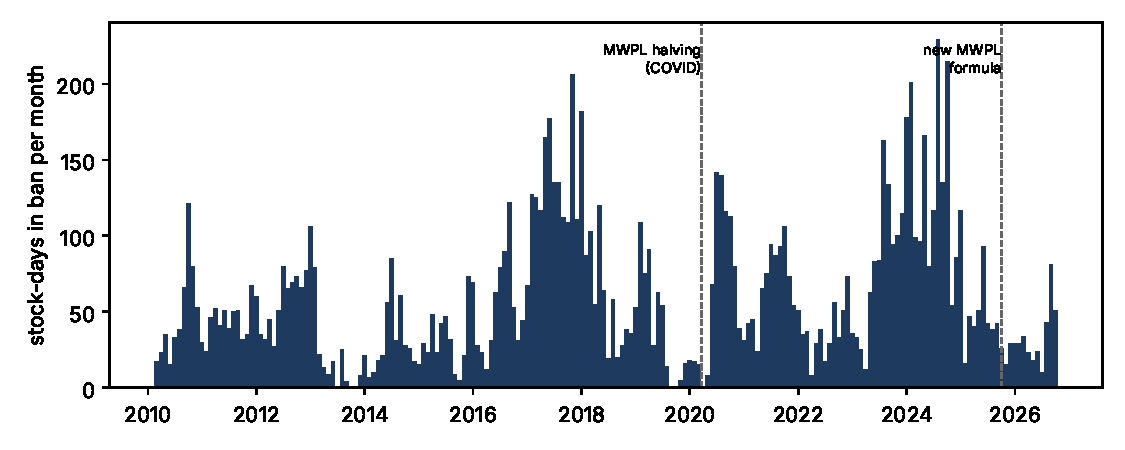
\includegraphics[width=0.9\textwidth]{ban_days_per_month.pdf}
\caption{Stock-days in the F\&O ban per month, 2010 to 2026.}\label{fig:bandays}
\end{figure}
\begin{figure}[h]\centering
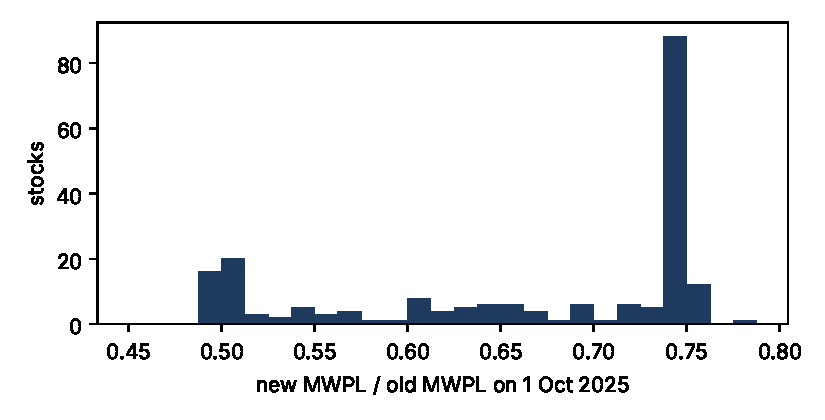
\includegraphics[width=0.6\textwidth]{mwpl_ratio_oct2025.pdf}
\caption{Ratio of the new to the old MWPL on 1 October 2025, all F\&O stocks.}\label{fig:mwpl}
\end{figure}

\section{The basis}
For each stock and day, the basis is computed from the volume-weighted average prices of the future and of the stock, net
of dividends going ex before expiry and of carry at the three-month interbank rate:
\[ m_{it}=\ln\bar F_{it}-\ln\big(\bar S_{it}-\mathrm{PV}_{it}(D)\big)-r_t\tau_{it}. \]
The near-month contract is used, switching to the next month when three or fewer trading days remain; at least five
contracts must trade; contracts with a dividend or other corporate event in their life and the first 20 trading days after
a stock enters the F\&O segment are excluded; the basis is winsorised at 1\% and 99\% within each year. The resulting sample
has 486,040 stock-days for 371 stocks, 8,851 of them in a ban. On the clean sample the median basis is $+1.2$\bp, and the
10th and 90th percentiles are $-33.0$ and $+26.2$\bp; the lower tail is wider than the upper. The basis shrinks toward
expiry. A relative implied repo rate (the stock's implied financing rate minus the day's cross-sectional median) and a
basis built from closing prices are used as checks.

\section{Other outcomes}
\begin{itemize}
\item \emph{Trading:} futures contracts traded (near and next month), the change in open interest in contracts, the ratio
$R=(\Delta OI+V)/V$, cash volume and the delivery share.
\item \emph{Earnings drift:} the buy-and-hold return over days $+2$ to $+64$ after a results announcement minus that of the
stock's size-decile portfolio; the surprise is the abnormal return over days $-1$ to $+1$; bad (good) news is the bottom
(top) tercile within each quarter. Returns are adjusted for splits, bonuses and dividends (the exchange's previous-close
field is not), and events with a price below Rs 5 are excluded.
\item \emph{Price delay:} the share of a stock's weekly return variation explained by lagged market returns (Hou and
Moskowitz, 2005), by calendar year.
\end{itemize}

\section{A constraint index for all stocks}\label{sec:index}
To measure how hard arbitrage is in each stock without using the outcomes or the treatments, I build a quarterly index for
all NSE stocks (80,042 stock-quarters, 3,310 stocks, 2015 to 2026) from five frictions: no short channel (not in the F\&O
segment), SLB scarcity (share of days without any SLB trade), the Corwin and Schultz (2012) spread, Amihud (2002)
illiquidity and idiosyncratic volatility. Each is standardised within the quarter, and the index is their first
principal component, which explains 53\% of their variance; all five load positively (0.37 to 0.49) and the loadings are
stable from year to year. The index is persistent (quarter-to-quarter rank correlation 0.90).

\begin{table}[h]\centering\small
\caption{Validation of the constraint index (frictions measured before outcomes)}\label{tab:index}
\begin{tabular}{lccc}
\toprule
Outcome & Per s.d.\ (s.e.) & Size-controlled & Obs. \\
\midrule
Price delay, next year (year FE) & $+0.058$ (0.003) & $+0.036$ (0.004) & 15,790 \\
Price delay, next year (stock and year FE) & $+0.032$ (0.005) & $+0.028$ (0.006) & 15,790 \\
Absolute drift after announcements & $+0.023$ (0.001) & $+0.015$ (0.001) & 69,673 \\
Drift after bad news & $-0.008$ (0.001) & $-0.001$ (0.002) & 23,219 \\
Drift after good news & $+0.001$ (0.001) & $+0.001$ (0.002) & 23,095 \\
\bottomrule
\end{tabular}

\vspace{2pt}\parbox{0.92\textwidth}{\footnotesize FE: fixed effects. Size control: log market capitalisation for price delay (15,227 stock-years with a market capitalisation); market-capitalisation decile fixed effects for drift.}
\end{table}
More constrained stocks respond more slowly to market news, also within a stock over time and after controlling for size,
and drift more after announcements in either direction (Table~\ref{tab:index}). Without a size control, drift after bad
news, but not good news, is stronger for more constrained stocks; with size-decile fixed effects this asymmetry disappears,
so it reflects the smaller size of constrained stocks rather than the short-sale constraint. These are associations. Within F\&O stocks, the short-channel component does not vary and SLB activity
appears to reflect demand to borrow rather than ease of borrowing, so for the futures-cash band of F\&O stocks I use a
separate F\&O index that adds utilisation of the position limit (Chapter~\ref{ch:band}).

\chapter{The no-arbitrage band: costs, capital and position limits}\label{ch:band}
\chapterlead{The band within which the basis moves in normal times, and how it relates to the three slow-moving limits:
trading costs, arbitrage capital and the position-limit regime. The chapter uses non-ban stock-days only, except where it
counts bans.}

\section{Estimating the band}
Let $x_{t-1}$ be yesterday's basis minus the stock's median basis on non-ban days, in basis points, and $\Delta m_t$ the
change in the basis of the same contract. The three-regime threshold model is
\[ \Delta m_t=a_r+\rho_r x_{t-1}+e_t,\qquad r=\begin{cases}\text{lower} & x_{t-1}<g_L\\ \text{middle} & g_L\le x_{t-1}\le g_U\\ \text{upper} & x_{t-1}>g_U,\end{cases} \]
with the thresholds chosen to minimise the sum of squared residuals over a grid of percentiles of $x$ (at least 10\% of
observations in each outer regime and 20\% in the middle). Linearity is tested with a sup-$F$ statistic whose distribution
under the linear model comes from a wild bootstrap clustered by date; threshold intervals come from resampling whole
stocks. I also estimate exponential and logistic smooth-transition models (Tse, 2001), in which the speed of reversion
changes smoothly with the deviation, and models in which it changes smoothly with an observed state.

\begin{table}[t]
\caption[Pooled threshold model of the basis]{The basis moves in a wide, asymmetric band, but much of the daily reversion is noise}\label{tab:setar}
\exsub{Pooled three-regime threshold model, non-ban days, 2015 to 2026 (473,110 observations, 360 stocks)}
\small\begin{tabular}{@{}>{\raggedright\arraybackslash\bfseries\color{accent}}p{6.4cm}ccc@{}}
\toprule
& \thd{Lower regime} & \thd{Middle regime} & \thd{Upper regime} \\
\midrule
Threshold (bp, relative to the stock's median) & below $-34.5$ & & above $+23.9$ \\
95\% interval (stock bootstrap) & $[-37.2,\,-32.2]$ & & $[+20.3,\,+26.1]$ \\
Share of observations & 0.12 & 0.76 & 0.12 \\
Slope of $\Delta m_t$ on $x_{t-1}$ & $-0.084$ & $-0.468$ & $-0.809$ \\
Slope, instrumented by $x_{t-2}$ & $-0.121$ & $-0.192$ & $-0.141$ \\
\bottomrule
\end{tabular}
\exsource{Thresholds chosen by least squares over a grid of percentiles; intervals from resampling whole stocks. Source: author's calculations.}
\end{table}

\begin{figure}[t]
\caption[Daily change in the basis against its deviation]{The further the basis moves from the stock's median, the more it reverts the next day}\label{fig:bandscatter}
\exsub{Mean change in the basis today by yesterday's deviation from the stock's median (5\bp\ bins), non-ban days; shaded: the estimated band}
\centering\includegraphics[width=\linewidth]{fig_band_scatter}
\exsource{Source: author's calculations.}
\end{figure}

Linearity is rejected (sup-$F$ 7,471 against a bootstrap 95\% critical value of 31). The band is about 58\bp\ wide and
asymmetric: the lower edge is further from the centre, as expected when reverse arbitrage is costlier than cash-and-carry.
By the Bayesian information criterion the threshold model fits best, the logistic smooth-transition model (slow reversion
below $+5$\bp, fast above) almost as well, and the symmetric exponential model clearly worse; a symmetric smooth transition
does not suit an asymmetric band.

The slopes need care. Inside the band the model of Chapter~\ref{ch:theory} predicts almost no correction, yet the middle
slope implies a half-life of about one day. Daily volume-weighted prices contain noise, and classical noise biases these
slopes toward $-1$. Instrumenting $x_{t-1}$ with $x_{t-2}$ (last row of Table~\ref{tab:setar}, with regimes classified by
$x_{t-2}$) shrinks all three slopes and removes most of the difference between the upper and lower regimes. Much of the
day-to-day reversion is therefore noise, and the slower reversion of cheap futures in the threshold model is not a robust
finding. The thresholds, which describe where the basis spends its time, are less affected.

\begin{figure}[t]
\caption[Estimated band edges by year]{The band is stable from year to year, apart from the dislocation of March 2020}\label{fig:bandyears}
\exsub{Thresholds of the pooled threshold model by calendar year, non-ban days, basis relative to each stock's median}
\centering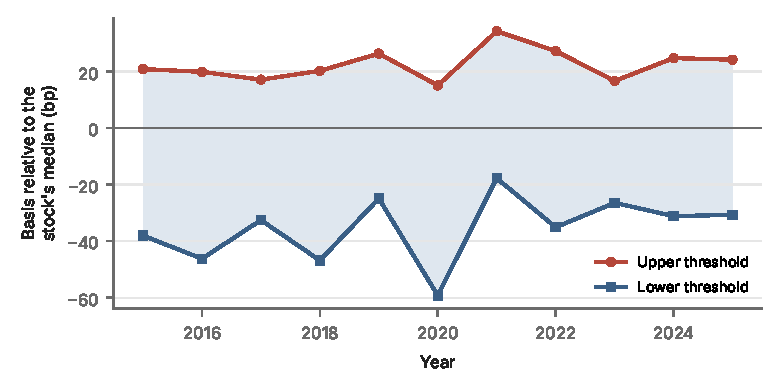
\includegraphics[width=\linewidth]{fig_band_years}
\exsource{Source: author's calculations.}
\end{figure}

The band is stable across years (Figure~\ref{fig:bandyears}), apart from 2020, when the March dislocation pushed the lower
edge to $-59$\bp. The lower edge is wider far from expiry ($-40$\bp\ with 17 or more trading days left against $-28$\bp\
in the last ten days), in line with edges that shrink as expiry approaches. In a smooth-transition model with the number
of trading days to expiry as the state, reversion is faster in the last week (the slope rises by 0.22 above seven days,
s.e.\ 0.02).

\section{Costs}
\paragraph{Pre-specified test (H3).} Around each STT increase I compare each stock's 80th percentile of the basis in the 40
trading days before and the 40 from the event.
\begin{table}[t]
\caption[Change in stock-level percentiles of the basis around STT increases]{The upper part of the basis rose after the 2024 and 2026 tax increases}\label{tab:h3}
\exsub{Mean change in each stock's percentiles of the basis, 40 trading days after against 40 before (bp)}
\small\begin{tabular}{@{}>{\bfseries\color{accent}}lccccc@{}}
\toprule
\thd{Event} & \thd{STT change} & \thd{Stocks} & \thd{80th percentile} & \thd{20th} & \thd{Median} \\
\midrule
3 Apr 2023$^{a}$ & $+0.25$ & 181 & $-2.12$ & $+0.24$ & $+0.27$ \\
1 Oct 2024 & $+0.75$ & 172 & $+6.42$ & $+4.55$ & $+5.39$ \\
1 Apr 2026 & $+3.0$ & 192 & $+7.44$ & $+2.10$ & $+6.30$ \\
\bottomrule
\end{tabular}

\exsource{$^{a}$ Same day as the change in the taxation of debt funds; reported, not used as evidence. STT change in bp of the futures sale. Source: author's calculations.}
\end{table}
Pooling 2024 and 2026, the mean change in the 80th percentile is $+6.96$\bp\ (s.e.\ 0.61, clustered by stock), and the
ordering of the three events matches the size of the cost changes. On the pre-specified statistic H3 is supported. The
pre-specified placebo, the same statistic at 30 dates away from the true events, tells a more cautious story: shocks common
to all stocks move the whole distribution, the placebo statistic has a standard deviation of 7.4\bp, and the true changes
rank at the 10th and 7th percentiles of the placebo distribution (Figure~\ref{fig:h3placebo}). The changes in the band's width and in the upper
percentile relative to the median are not unusual. The rise is mostly a shift of the whole distribution, larger than the
cost changes, and standard errors clustered only by stock overstate the precision when every observation shares the same
event date (Kolari and Pynn\"onen, 2010).

\begin{figure}[t]
\caption[The STT events against placebo dates]{Against placebo dates, the rise after the tax increases is large but not exceptional}\label{fig:h3placebo}
\exsub{Mean change in stocks' 80th percentile of the basis at the three STT dates and at 30 placebo dates (bp)}
\centering\includegraphics[width=\linewidth]{fig_h3_placebo}
\exsource{Placebo dates every 80 trading days, away from the true events. Source: author's calculations.}
\end{figure} As a further check, the same statistic at the three dates of SEBI's 2024 to 2025
reforms of index derivatives, which did not change the costs of single-stock arbitrage, gives $-4.1$, $-0.3$ and
$+1.9$\bp, all well inside the placebo range.

\paragraph{Band edges by tax period.} Measuring each deviation from the stock's median within each period (the full-sample
median does not remove the 2026 level shift), the upper threshold is $+23.8$, $+18.9$, $+23.1$ and $+28.9$\bp\ in the four
STT periods and the lower threshold $-39.1$, $-30.9$, $-31.5$ and $-31.5$\bp. The upper edge is highest in the
highest-tax period but does not rise step by step with the tax. Reversion above the upper edge weakens over time (slope
$-0.77$, $-0.55$, $-0.20$, $-0.15$), which coincides with both rising costs and rising arbitrage capital.

\paragraph{A bottom-up cost band.} The full round trip of an overnight cash-and-carry position (STT of 0.1\% on the cash
purchase and on delivery at expiry, STT on the futures sale, stamp duty, exchange charges, the SEBI fee, GST and an
institutional brokerage of 0.01\% per leg) costs 27.1, 27.3, 28.0 and 31.0\bp\ in the four periods (25 to 38\bp\ for
brokerage between 0.005\% and 0.03\% per leg). Rolling an existing position for one more month costs 4.0 to 8.0\bp. The
estimated upper threshold in levels ($+22$ to $+28$\bp) and the 80th percentile lie below the full round trip, which sits
between the 90th and 95th percentiles. New capital enters only at large deviations; funds that keep capital in place and
roll can lean against much smaller ones. This is one reason why fixed thresholds sit inside the full cost band, as the
model's inventory result implies (Figure~\ref{fig:costband}).

\begin{figure}[t]
\caption[The bottom-up cost of a cash-and-carry position]{The full cost of a new position lies above the estimated upper edge}\label{fig:costband}
\exsub{Round trip of an overnight cash-and-carry position held to delivery, by STT period (bp of notional); triangles: estimated upper threshold in levels}
\centering\includegraphics[width=\linewidth]{fig_cost_band}
\exsource{Institutional brokerage of 0.01\% per leg; GST of 18\% on fees and brokerage. Source: NSE circulars on STT and transaction charges; author's calculations.}
\end{figure}

\section{Arbitrage capital}
\paragraph{Pre-specified test (H4).} Monthly, from May 2018 to September 2026, I regress the 80th percentile of the basis
across all non-ban stock-days on last month's net inflow into arbitrage funds as a share of their assets, with step
dummies for April 2023, October 2024 and April 2026. The coefficient is $-17.5$\bp\ per unit of flow (Newey-West s.e.\ 14.2,
one-sided $p=0.11$): a 10\% inflow goes with a 1.7\bp\ lower upper quantile the next month. In first differences the
relation is clearer ($-20.6$, s.e.\ 6.8), and it is visible before April 2023 ($-26.0$, s.e.\ 16.5) but not after
($+17.1$, s.e.\ 16.9). Same-month flows have a positive coefficient, as expected when flows chase the returns that a rich
basis offers. With about a hundred months the test has little power (Figure~\ref{fig:h4}).

\begin{figure}[t]
\caption[Arbitrage-fund flows and the upper tail of the basis]{The upper tail of the basis and arbitrage-fund flows move a great deal from month to month}\label{fig:h4}
\exsub{Monthly 80th percentile of the basis across non-ban stock-days (top) and net inflow into arbitrage funds as a share of assets (bottom); dashed: April 2023}
\centering\includegraphics[width=\linewidth]{fig_h4_flows}
\exsource{Source: AMFI monthly reports; NSE bhavcopies; author's calculations.}
\end{figure}

\paragraph{Capital as a state.} In a smooth-transition model with log arbitrage-fund assets as the state, reversion is
faster when assets are large (the slope falls by 0.077, s.e.\ 0.019, above about Rs 95,000 crore). This variable also orders
time, so the evidence is descriptive.

\paragraph{Peak margins.} From December 2020 to September 2021 margins had to be collected on peak intraday positions, in
four steps of 25\%. This raises the capital an arbitrageur must post during the day. The upper percentile moves in both
directions at the four steps ($+3.3$, $+9.6$, $-9.9$ and $+3.5$\bp, against a placebo standard deviation of 7.4), so I find
no consistent effect; the rule mainly binds intraday leverage, which a daily basis does not measure.

\section{Position limits}
\paragraph{Anticipation (H9).} On non-ban days before October 2025, the share of days on which a stock's basis is in its own
upper tail (above the 80th percentile of its days with utilisation below 60\%) rises from 0.20 to about 0.27 as utilisation
the day before approaches 95\% (Figure~\ref{fig:h9}). With stock and date fixed effects, the slope of this share on
utilisation between 0.60 and 0.95 is $+0.079$ (s.e.\ 0.038, one-sided $p=0.019$), the lower tail does not change, and the
increase comes more as a step around 0.75 than as a smooth slope. The basis is more often rich as the trigger nears, as
the anticipation result predicts, although high utilisation also signals demand pressure. In a smooth-transition model
with utilisation as the state, reversion weakens as utilisation rises (the slope rises by 0.225, s.e.\ 0.053).

\begin{figure}[t]
\caption[The basis as utilisation nears the trigger]{Rich futures become more common as utilisation approaches the 95\% trigger}\label{fig:h9}
\exsub{Share of non-ban days with the basis in the stock's upper and lower tail, by utilisation the day before (raw shares, before October 2025)}
\centering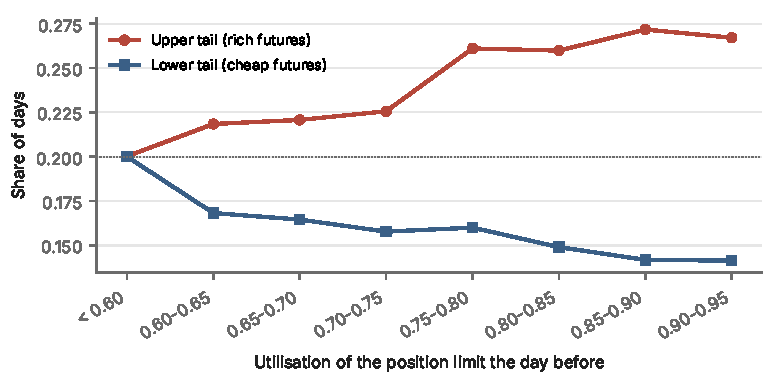
\includegraphics[width=\linewidth]{fig_h9_tails}
\exsource{With date fixed effects the lower-tail decline disappears; the upper-tail rise remains. Source: author's calculations.}
\end{figure}

\paragraph{The October 2025 formula and quarterly resets.} The size of each stock's MWPL cut on 1 October 2025 (0.24 to
0.69 log points) raised its utilisation strongly (first stage $+0.28$ per unit, s.e.\ 0.03). Its effect on the upper tail is
$+0.061$ (s.e.\ 0.050, $p=0.11$), on the level $+4.8$\bp\ and on bans $+0.023$: all in the predicted direction, none
significant. The quarterly resets of January, April and July 2026 move utilisation but show no effect on the basis.

\paragraph{How the October 2025 rules changed the number of bans.} SEBI's stated aim was to reduce ``spurious'' bans. Before
the reform, bans were driven by open interest, not by changes in the limit: on the day utilisation crossed 95\% the limit
fell for only 8 of 1,744 entries, and only 7 (0.4\%) would not have crossed at the previous day's limit. To see what the
two parts of the reform did, I simulate the ban rule (enter the day after utilisation exceeds 95\%, leave the day after it
is at or below 80\%) for the stocks that were in the segment on both 30 September and 1 October 2025. Applied to the actual
utilisation, the simulation reproduces the official ban lists exactly. I then apply it with open interest measured gross
or in delta terms, and with the new limit or the limit the old formula would have given (each stock's new limit scaled by
its ratio of old to new limit on 1 October 2025, an approximation).

\begin{table}[t]
\caption[Bans under the new rule and under counterfactual rules]{The new rule produced about a quarter of the ban days the old rule would have}\label{tab:spurious}
\exsub{Bans from 1 October 2025 to 27 October 2026 for the stocks in the segment on 30 September and 1 October 2025}
\small\begin{tabular}{@{}>{\bfseries\color{accent}}lccc@{}}
\toprule
\thd{Open interest and limit} & \thd{Ban stock-days} & \thd{Spells} & \thd{Stocks} \\
\midrule
Delta-adjusted, new limit (the actual rule) & 412 & 45 & 11 \\
Gross, old-formula limit (the old rule) & 1,505 & 112 & 36 \\
Gross, new limit & 6,256 & 296 & 85 \\
Delta-adjusted, old-formula limit & 1 & 1 & 1 \\
\bottomrule
\end{tabular}

\exsource{The 45 spells include one that began on 30 September 2025. Simulated ban rule validated against the official lists. Source: NSE combined open interest files; author's calculations.}
\end{table}

\begin{figure}[t]
\caption[Ban days under four rules]{Measuring open interest in delta terms removes almost all bans; the lower limit alone would have multiplied them}\label{fig:spurious}
\exsub{Ban stock-days, 1 October 2025 to 27 October 2026, under the actual and three counterfactual rules}
\centering\includegraphics[width=\linewidth]{fig_spurious}
\exsource{Source: as for Table~\ref{tab:spurious}.}
\end{figure}

Under the old rule the same stocks would have spent about 3.7 times as many days in a ban (Table~\ref{tab:spurious}).
The two parts of the reform pull in opposite directions: measuring open interest in delta terms removes almost every
ban, because options now count only by their delta and offsetting positions of the same client net out, while the lower limit on its own would have quadrupled them.
The combination cut bans by about three quarters.

\paragraph{The 2020 halving and restoration.} From 23 March 2020 the limit was halved for stocks whose recent daily
price range or utilisation was high, and on 27 November 2020 it was restored for the 70 stocks whose limit was then
halved. The restoration is a clean shock: it was
announced, it came in a calm market, and it doubled the limit of some stocks and not others. Against other F\&O stocks, in
the 40 trading days either side, the utilisation of the restored stocks fell by 0.21 (s.e.\ 0.02), their share of days in
a ban by 4.6 percentage points (s.e.\ 1.4), and the share of days with their basis in its upper tail by 6.8 percentage
points (s.e.\ 3.2). The basis level did not change significantly ($-2.8$\bp, s.e.\ 3.1). A false restoration date 20 days
earlier shows no effect on utilisation, bans or the upper tail. A looser limit makes rich futures less common, as the
anticipation result predicts, although the upper-tail effect is weaker with a 20-day window ($-6.1$, s.e.\ 4.0). The
halving itself coincided with the March 2020 crash and selected stocks on the outcomes, so I do not interpret it.

\begin{figure}[t]
\caption[The 2020 restoration of the position limit]{Restoring the limit cut the utilisation of the affected stocks at once}\label{fig:covid}
\exsub{Mean utilisation of the MWPL for the 70 stocks whose limit was restored on 27 November 2020 and for other F\&O stocks}
\centering\includegraphics[width=\linewidth]{fig_covid}
\exsource{The fall on day 0 is mechanical (the denominator doubled); the tests use bans and the basis. Source: NSE combined open interest files; author's calculations.}
\end{figure}

\section{Frictions across stocks (H1)}
For F\&O stocks I build a quarterly friction index from the spread, illiquidity, idiosyncratic volatility, utilisation of
the position limit and SLB scarcity, measured in the previous quarter. A one standard deviation higher index goes with a
band (80th minus 20th percentile of the basis) 3.5\bp\ wider (s.e.\ 1.1, one-sided $p=0.002$; mean 40.8\bp) and a mean
absolute basis 2.5\bp\ larger. The relation is across stocks: with stock fixed effects it disappears. The persistence
measure moves the wrong way, which the noise result above explains, and SLB scarcity enters with the wrong sign, which
suggests that SLB activity reflects demand to borrow. Per-stock threshold models (258 stocks) give a median band of $-26$ to
$+17$\bp, and their widths are not related to the stocks' average index.

\section{Summary}
The basis follows a wide, asymmetric, nonlinear band. Its edges respond to costs less cleanly than the model implies; the
full cost of new arbitrage lies in the outer tail, while the cost of keeping capital in place is small. Capital and the
position-limit regime leave traces in the predicted direction (faster correction with more capital, a richer basis near
the trigger, a less often rich basis after the 2020 restoration of the limit), but the formal tests of capital flows and of
the 2025 reform are not significant. The 2025 rules cut the number of bans by about three quarters.

\chapter{The F\&O ban}\label{ch:ban}

\section{Trading in a ban (H8)}
I compare each stock's ban days with its own non-ban days at similar utilisation the day before (80\% to 95\%, the only
range in which both occur), before October 2025, excluding expiry days, with stock-by-utilisation-bin and date fixed effects
and standard errors clustered by stock and date.
\begin{table}[h]\centering\small
\caption{Effect of a ban on trading}\label{tab:h8}
\begin{tabular}{lcc}
\toprule
Outcome & Effect (s.e.) & Non-ban mean \\
\midrule
log(1 + futures contracts traded) & $-2.00$ (0.11) & \\
log(1 + cash shares traded) & $+0.073$ (0.027) & \\
Delivery share of cash volume & $+0.041$ (0.005) & 0.26 \\
\bottomrule
\end{tabular}
\end{table}
Futures trading falls by about 87\%, cash volume rises by about 7.5\% and more of it is delivered (Table~\ref{tab:h8}). H8
is supported.

The model also predicts that if the rule binds trade by trade, the change in open interest equals minus the volume, so
$R=(\Delta OI+V)/V$ is zero on ban days (it is about one on normal days). Over the whole period the ban-day mean of $R$ is
0.42, so the identity fails on the pre-set reading. The explanation lies in enforcement (Figure~\ref{fig:R}): until 22 March
2020, when violations were judged on end-of-day positions, the median ban-day $R$ is 0.87; from 23 March 2020, when the
clearing corporations judged violations on peak intraday positions, it is 0.011; under the delta-based rule from October
2025 it is 0.19 to 0.36. When the rule binds trade by trade, the identity holds almost exactly. The effect of a ban on
futures volume is $-0.97$ log points before March 2020 and $-2.72$ after.

\begin{figure}[h]\centering
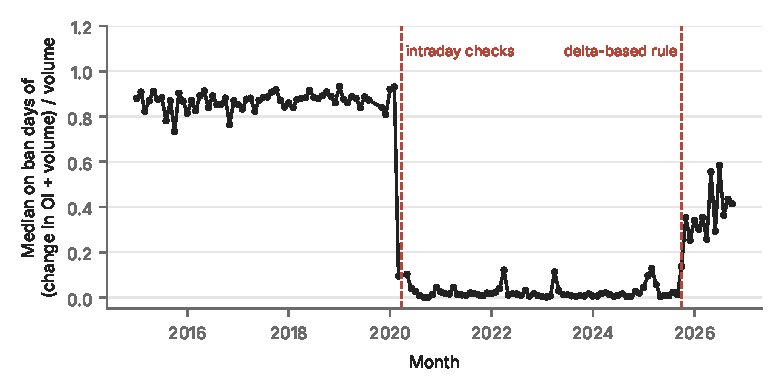
\includegraphics[width=0.75\textwidth]{fig_ban_R.pdf}
\caption{Monthly median of $(\Delta OI+V)/V$ on ban days (near and next futures, expiry days excluded).}\label{fig:R}
\end{figure}

\section{Does correction become one-sided? (H7)}
I regress the daily change in the basis on yesterday's deviation from the stock's median, separately in an upper regime
(above the stock's 80th percentile on non-ban days), a middle and a lower regime (below the 20th percentile), and let each
slope change on ban days. The model predicts that upward deviations revert more slowly in a ban ($\delta_{up}>0$) and
downward deviations as fast or faster.
\begin{table}[h]\centering\small
\caption{Reversion of the basis by regime, and its change in a ban}\label{tab:h7}
\begin{tabular}{lcc}
\toprule
& Normal slope (s.e.) & Change in a ban (s.e.) \\
\midrule
Upper regime & $-0.712$ (0.010) & $-0.089$ (0.037) \\
Middle & $-0.393$ (0.026) & $+0.099$ (0.062) \\
Lower regime & $-0.204$ (0.010) & $+0.081$ (0.030) \\
\bottomrule
\end{tabular}
\end{table}
The prediction fails, with the opposite sign: in a ban rich futures revert faster and cheap futures more slowly
(Table~\ref{tab:h7}). This holds with other threshold definitions, without imputed ban days and with the relative implied
repo rate; with the close-based basis the upper change is about zero. It is stronger on liquid days, differs by
enforcement period, and is concentrated in the first days of a spell ($-0.163$ in the first five calendar days against
$-0.008$ later). Instrumenting yesterday's deviation with the deviation two days earlier, to remove the effect of noise in
daily prices, gives $-0.190$ (s.e.\ 0.077) for the upper regime and $+0.088$ (0.015) for the lower: the result is not
caused by noisier prices on ban days.

A reading consistent with these facts, though not tested in advance, is that at the start of a ban the model's second
channel dominates: demand for new futures exposure is blocked, which removes the pressure that had made futures rich, so
upward deviations close quickly. The prediction tested was derived from the reduce-only arbitrage channel alone.

\section{The level of the basis when a ban starts}
\paragraph{Design.} Each ban spell from 2015 to September 2025 with no ban in the five days before it is an event. Controls
are other stocks in the same week with utilisation between 85\% and 95\% and no ban within five days, matched (up to five,
nearest by Mahalanobis distance) on the utilisation path of the previous five days and the basis on the day before. The
outcome is the change in the basis from the day before the ban, treated minus matched controls, averaged over the ban days
among the first five. Composition $C$ is the change in futures open interest over the five days before entry divided by
futures volume.

\paragraph{Results.} Over 889 matched entries the basis falls by 6.3\bp\ on average (median $-7.8$). With falling open
interest before entry ($C\le0$, 30 events) it rises by 8.4\bp\ (s.e.\ 10.9); with rising open interest it falls by 6.8\bp\
(s.e.\ 1.8). The difference, the pre-specified statistic, is $-15.2$\bp\ (one-sided $p=0.083$): the signs are those of the
model's level result, but the closing-pressure group is small because open interest must rise for utilisation to cross
95\%. Splitting at the median of $C$ instead gives a difference of $-5.8$ (s.e.\ 2.9, $p=0.025$), and $C$ as a continuous
variable gives $-4.8$ per standard deviation (s.e.\ 1.6, $p=0.001$). The basis returns to its earlier level about a week
after the start (Figure~\ref{fig:level}).

\begin{figure}[h]\centering
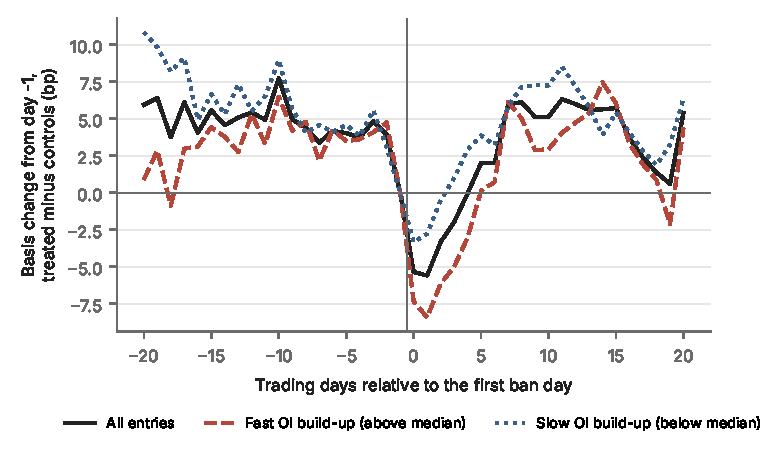
\includegraphics[width=0.8\textwidth]{fig_level_profile.pdf}
\caption{Change in the basis from the day before a ban starts, treated minus matched controls, by event time.}\label{fig:level}
\end{figure}

\paragraph{Caveats.} The matching leaves the treated basis 10\bp\ below that of the controls on the day before, and the
treated basis dips on that day; with the baseline taken over days $-10$ to $-2$, or controlling for the gap, the in-ban fall
is 9 to 11\bp\ and the composition slope stays negative. With controls from the same day only (685 events) the fall is
$-4.0$\bp\ (s.e.\ 2.0) but the composition gradient is not significant. Classifying events instead by the direction of
open interest and price (long build-up, short build-up, short covering, long unwinding), the in-ban fall appears for both
long build-up ($-7.9$\bp) and short build-up ($-5.5$\bp), so it is not specific to new long demand.

\section{The 95\% trigger}
\paragraph{Density.} Among stocks that were below 95\% the day before, the density of today's utilisation is smooth through
the trigger (Figure~\ref{fig:density}; Cattaneo, Jansson and Ma test, $T=-0.18$, $p=0.86$), across polynomial orders,
bandwidths and enforcement periods. Utilisation accelerates rather than stalls near the trigger: its mean daily change
is larger just below 95\%, and the share of stocks crossing the next day rises steadily to about one half at 0.93 to 0.95.
There is no sign that traders hold back to avoid a ban.

\begin{figure}[h]\centering
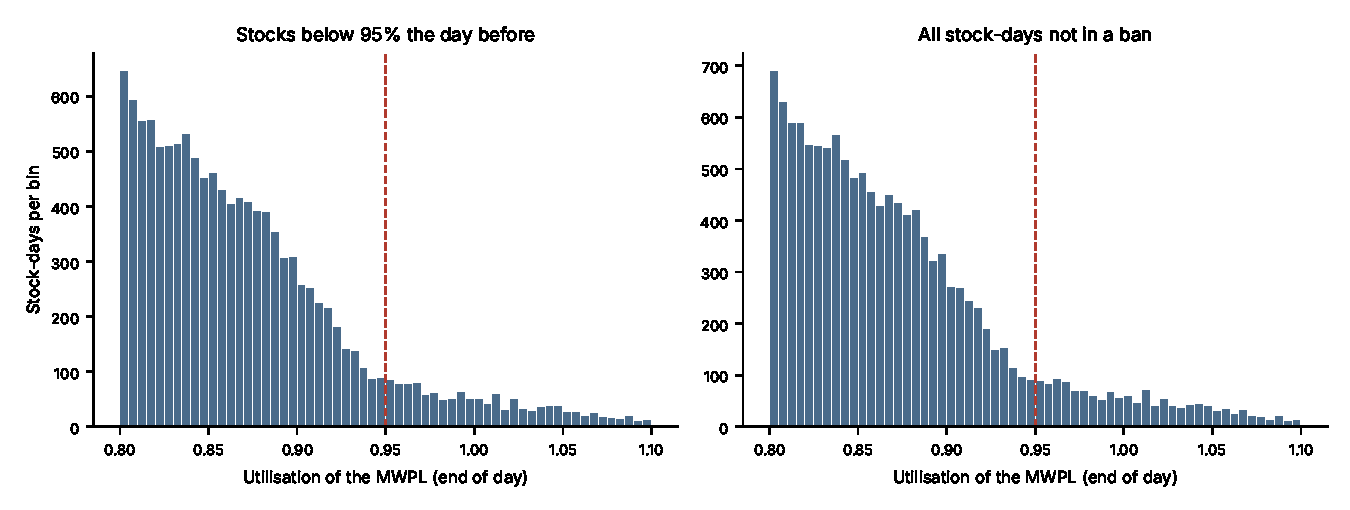
\includegraphics[width=0.85\textwidth]{density_95.pdf}
\caption{Utilisation at the end of the day. Left: stocks that were below 95\% the day before. Right: all stock-days not in
a ban (this population thins above 95\% by construction, because stocks above the trigger are in the ban the next day).}\label{fig:density}
\end{figure}

\paragraph{Regression discontinuity.} For stocks not in a ban the day before, crossing 95\% puts the stock in the ban the
next day in 99.7\% of cases. Local linear estimates with robust bias-corrected inference show sharp jumps in trading:
futures contracts $-1.53$ log points, $R$ $-0.66$, delivery share $+0.051$; cash volume does not jump. The basis level is
12.9\bp\ lower above the cutoff ($p=0.02$), but the basis is already 11.3\bp\ lower on the crossing day itself, before the ban
starts, and the change on the first ban day is small ($-2.8$, s.e.\ 4.1). The discontinuity therefore confirms the trading
mechanism but cannot separate a level effect of the ban from the pressure that pushes utilisation over the trigger.

\paragraph{Hysteresis.} Between 80\% and 95\% utilisation, stocks in a ban and stocks not in a ban can be compared at equal
utilisation. Controlling for utilisation, its change, five lags of the basis and stock and date fixed effects, being in a
ban changes the basis by $+0.4$\bp\ (s.e.\ 0.8, $p=0.64$); without the lags the difference is $-14.1$\bp. Banned stocks carry
the low basis of the start of the spell; the reduce-only state does not shift it further. Its effect on trading is as
strong as in H8.

\section{Bad news in a ban (H2)}
Of 8,586 results announcements of F\&O stocks, 179 fall on ban days, 55 of them bad news, so this test has little power, as
stated in advance. The drift after bad news is $-1.25\%$ outside bans relative to the middle tercile; in bans the additional
effect is $+0.7\%$ (s.e.\ 3.4). Outside bans the basis over the five days before an announcement is 2.0\bp\ lower before bad
news than before good news (s.e.\ 1.1, one-sided $p=0.04$), the pattern reported by Saurav, Srivastava and Agarwalla (2026);
inside bans the difference cannot be estimated with useful precision.

\section{Summary}
Bans bind hard on trading, and the identity that every trade closes positions holds once the rule is enforced on intraday
positions. The basis does not behave as the reduce-only arbitrage channel alone predicts: rich futures revert faster, and
the basis falls when a ban starts, more after fast build-ups of open interest. Both facts fit the model's second channel,
blocked new demand, but that reading was formed after seeing the results.

\chapter{F\&O eligibility and the cross-section}\label{ch:elig}
\chapterlead{Short-sale constraints across the whole cash market: what entry into and exit from the F\&O segment do to
price adjustment and drift, whether anomalies are stronger where shorting is hardest, and how drift and price delay vary
across all stocks.}

\section{Entry into and exit from the F\&O segment (H6)}
Entry gives a stock futures, options and formal short-selling eligibility at once; an eligibility exit removes them while
the stock keeps trading in the cash market. This changes the short-sale constraint for many more stocks than the ban
does, and against the whole cash market as a control group.

\paragraph{Design.} Stocks by calendar year, 2015 to 2025. A stock's cohort is the first year fully after its event; the
event year is a transition year. For price delay I use the Callaway and Sant'Anna (2021) estimator with never-treated and
not-yet-treated controls and base-year covariates (log market capitalisation, log traded value, volatility), with a
stock-cluster bootstrap. Drift exists only at announcements, so for drift after bad news I use a stacked
difference-in-differences at the announcement level. The family statistic is a Bonferroni combination of the four
components.

\begin{table}[t]
\caption[Effects of F\&O entry and exit]{Entry speeds price adjustment; drift after bad news does not weaken}\label{tab:h6}
\exsub{Pre-specified components of the H6 test}
\small\begin{tabular}{@{}>{\bfseries\color{accent}}lcccc@{}}
\toprule
\thd{Component} & \thd{Prediction} & \thd{Estimate} & \thd{s.e.} & \thd{One-sided $p$} \\
\midrule
Entry: price delay & $<0$ & $-0.109$ & 0.023 & $1.3\times10^{-6}$ \\
Entry: drift after bad news & $>0$ & $-0.040$ & 0.018 & 0.99 \\
Exit: price delay & $>0$ & $+0.053$ & 0.040 & 0.091 \\
Exit: drift after bad news & $<0$ & $+0.014$ & 0.020 & 0.77 \\
\bottomrule
\end{tabular}
\exsource{Price delay: Callaway and Sant'Anna estimator, stock-cluster bootstrap. Drift: stacked difference-in-differences at the announcement level. Source: author's calculations.}
\end{table}

Prices of stocks that enter the segment respond much faster to market-wide news (median delay 0.24 before entry), and those
of stocks that leave somewhat more slowly. The Sun and Abraham (2021) estimator gives $-0.063$ (s.e.\ 0.019) for entries,
leads three and four years before entry are close to zero, and the result holds without the large November 2024 batch and
without back-cast market capitalisations. The drift components go the other way: after entry the drift that follows bad
news is stronger, not weaker. H6 is supported through price delay and contradicted through drift. Entry requires a stock
to have grown in size and liquidity, which by itself speeds price adjustment; the covariates and the flat leads limit,
but cannot rule out, selection on growth (Figure~\ref{fig:h6es}).

\begin{figure}[t]
\caption[Price delay around F\&O entry and exit]{Price delay falls after entry and rises a little after exit, with no clear trend before either}\label{fig:h6es}
\exsub{Callaway and Sant'Anna estimates of the change in price delay by year relative to the first full year after the event (cells with at least 19 treated stocks)}
\centering\includegraphics[width=\linewidth]{fig_h6_es}
\exsource{Point estimates; the aggregate post-event effects and their standard errors are in Table~\ref{tab:h6}. Source: author's calculations.}
\end{figure}

\section{Anomalies and short-sale constraints (H5)}
Each month I sort stocks within three constraint groups (F\&O stocks; cash-only stocks with SLB trades in the last three
months; cash-only stocks without) into terciles of a composite mispricing score built from momentum, short-term reversal,
maximum daily return, idiosyncratic volatility, illiquidity and turnover, and measure the most overpriced and most
underpriced terciles against the group's value-weighted return. The model predicts that the overpriced side does worse
where shorting is hardest, while the underpriced side does not differ.

Value-weighted, it does not: the short-leg difference between the most constrained group and F\&O stocks is $+0.04\%$ a
month (s.e.\ 0.20). Equal-weighted, anomalies are far stronger among small cash-only stocks, but on both sides (short leg
$-0.49\%$, long leg $+0.46\%$ a month relative to F\&O stocks), which is a small-stock effect rather than the one-sided
pattern of a short-sale constraint. Momentum alone fits the prediction: losers among constrained stocks do worse ($-0.51\%$
a month, s.e.\ 0.22). The groups differ greatly in size (median market capitalisation Rs 43,513 crore for F\&O stocks
against Rs 770 crore for cash-only stocks without SLB trades), which limits what this comparison can show
(Figure~\ref{fig:h5}).

\begin{figure}[t]
\caption[Anomaly returns where shorting is hardest]{Value-weighted, the overpriced side does no worse where shorting is hardest}\label{fig:h5}
\exsub{Most constrained group (cash-only stocks without SLB trades) minus F\&O stocks, short and long legs of a composite mispricing sort}
\centering\includegraphics[width=\linewidth]{fig_h5_legs}
\exsource{Newey-West standard errors; holding months January 2016 to September 2026. Source: author's calculations.}
\end{figure}

\section{Drift and price delay across all stocks}
Two further comparisons use the whole cash market. First, relative to F\&O stocks of the same size decile, cash-only stocks
drift $-0.67\%$ more after bad news (s.e.\ 0.42) and $+2.40\%$ more after good news (s.e.\ 0.43): they under-react in both
directions. Second, the constraint index of Chapter~\ref{ch:data}, which combines the lack of a short channel with SLB
scarcity, spreads, illiquidity and idiosyncratic volatility, predicts slower price adjustment the next year, also within a
stock over time and after controlling for size. It also predicts more drift after bad news than after good news, but that
asymmetry disappears once size is controlled for, in line with the symmetric under-reaction of cash-only stocks.

\section{Summary}
Short-sale access matters for how fast prices adjust: entry into the F\&O segment speeds the response to market news, and
more constrained stocks adjust more slowly. The evidence on overpricing and on drift after bad news is mixed: entry does
not weaken bad-news drift, value-weighted anomaly returns do not show the predicted asymmetry, and the link between the
broader constraint index and drift after bad news disappears once size is controlled for.

\chapter{Conclusion and policy}\label{ch:concl}

\section{What binds}
\begin{table}[h]\centering\small
\caption{The pre-specified tests}\label{tab:summary}
\begin{tabularx}{\textwidth}{>{\raggedright\arraybackslash}p{4.2cm}>{\raggedright\arraybackslash}p{3.2cm}L}
\toprule
Hypothesis & Pre-specified result & Comment \\
\midrule
\multicolumn{3}{l}{\emph{Primary family (Holm correction at 5\%)}} \\
H8: trading leaves futures in a ban & Supported ($p<10^{-10}$) & Identity holds under intraday enforcement \\
H3: costs set the band edges & Supported ($p<10^{-10}$) & Placebo-calibrated evidence weak; mostly a common shift \\
H6: short-sale access & Supported ($p=5\times10^{-6}$) & Through price delay; drift goes the other way \\
H7: one-sided correction & Rejected, opposite sign & Survives a noise correction \\
\midrule
\multicolumn{3}{l}{\emph{Secondary (unadjusted)}} \\
Level effect by composition & $p=0.083$ & Signs as predicted; median split $p=0.025$ \\
Density at 95\% & No discontinuity & No bunching \\
Regression discontinuity & Basis $-12.9$\bp, $p=0.02$ & Gap present before the ban \\
Hysteresis & $+0.4$\bp, $p=0.64$ & No extra level shift \\
H9 anticipation & $p=0.019$ & Upper tail grows toward 95\% \\
H9 reform & $p=0.11$ & Right direction \\
H2 bad news in bans & $p=0.59$ & No power \\
H1 frictions and band & $p=0.002$ & Across stocks only \\
H4 capital & $p=0.11$ & Clearer in differences \\
H5 anomalies & $p=0.57$ & Not supported value-weighted \\
\bottomrule
\end{tabularx}
\end{table}

The answer to the question this thesis asks is uneven across the limits. Position limits bind hard on trading: the ban
moves trading out of futures as soon as it is enforced on intraday positions. Their effect on prices is real but not the
one the reduce-only arbitrage channel predicts; the evidence points instead to the blocking of new demand at the start of
a ban. Short-sale access matters for how fast prices adjust to market news, both when a stock enters the F\&O segment and
across all stocks, but less clearly for overpricing. Trading costs shape the band, which is wide and asymmetric, but its
edges do not move one-for-one with the tax: the full cost of a new position lies in the outer tail of the basis, and the
cost of keeping arbitrage capital in place is small. Arbitrage capital leaves weak traces in the predicted direction.

With ten secondary statistics reported without adjustment, one or two values below 0.05 would be expected by chance. The
secondary results should be read as a pattern, not one by one.

\section{Policy}
Position limits and the ban exist to contain concentrated positions and manipulation in a market where speculative
demand is large. SEBI's study of individual traders in equity derivatives (SEBI, 2024a) shows how large: over the three
years to March 2024, 93\% of more than one crore individual traders lost money, on average about Rs 2 lakh each including
transaction costs, and their aggregate losses exceeded Rs 1.8 lakh crore. In the last of those years proprietary traders and
foreign portfolio investors earned gross profits, 96 to 97\% of them from algorithmic trading. SEBI's measures of October 2024 for index
derivatives cite the rise in retail participation and speculative volumes (SEBI, 2024b), and its measures of May 2025
changed how open interest is measured and how position limits are set (SEBI, 2025). Most of that
activity is in index options, not in the single-stock futures studied here, but the same pressure of new speculative
demand is what pushes a stock towards its limit.

The results bear on the trade-off in four ways. First, the ban is costly for liquidity: futures trading falls by almost
90\% in a ban, while cash trading rises a little. Second, its main price effect appears at the start of a ban, where it
fits the blocking of new demand, and fades within about a week; once a stock is in the ban, staying in it does not move
the basis further. If that reading is right, a ban restrains the demand it is designed to restrain, but at the cost of the
arbitrage that would otherwise keep futures and cash prices together. Third, enforcement matters: the rule changes trading in the way it
is meant to only when positions are checked during the day. The October 2025 rule, which allows any trade that lowers an
entity's end-of-day delta, has visibly loosened the link between volume and open interest in banned stocks.

Fourth, the 2025 reform met its stated aim of fewer ``spurious'' bans (SEBI, 2025, para.\ 4.2). Before the reform, bans
were not caused by falls in the limit: almost every entry came from rising open interest. What made many of them avoidable
was the measure of open interest, which counted every option at its full notional value. Measuring positions in delta terms
removes almost all of these bans, the new and lower limits add some back, and the combination cut ban days by about three
quarters in the first year. Whether the new formula has changed the cost of each ban needs more post-reform data than the
44 spells that began after the reform. The 2020 restoration of the limit adds one more lesson: a looser limit lowered
utilisation and bans and made a rich basis less common, so the level of the limit affects prices even before a ban starts.

The SLB market remains thin. Because only F\&O stocks may be sold short and the overnight short is in practice a stock
future, entry into and exit from the F\&O segment change the short-sale constraint of a stock at once. The faster price
adjustment after entry is one measurable benefit of that access.

\section{Limitations and further work}
The data are daily, so intraday arbitrage and the exact timing of trades within the day are outside the scope, and noise
in daily prices inflates measured reversion. Arbitrage inventory is not observed. The post-reform period is short. Three
papers relevant to positioning (Saurav, Srivastava and Agarwalla, 2026; Gagnon, 2018; Brennan and Schwartz, 1990) could
not be read in full. Intraday data would allow sharper tests of the ban's effect on correction, and a longer post-reform
sample would allow a proper test of the 2025 formula.


\appendix
\chapter{The pre-analysis plan and its log}\label{app:plan}

\section{The plan}
Before any outcome (basis, returns, drift, delay) was related to any treatment (ban status, utilisation, MWPL changes, STT
dates, F\&O entry or exit, the tax change), I wrote a pre-analysis plan fixing the samples, the outcome and treatment
definitions, the specifications, the predicted signs, the falsifiers, the inference and the primary and secondary
hypotheses. It was frozen with a time-stamped tag in the project's version control on 5 November 2026, after the guide's
go-ahead and a full audit of the data. Until then, only treatment-side counts and outcome distributions on their own had
been examined.

\begin{itemize}
\item \emph{Primary family:} H7 (one-sided correction), H8 (trading), H3 (costs and band edges), H6 (F\&O entry and exit),
corrected jointly by the Holm method at 5\%.
\item \emph{Secondary tests:} the level effect, H9, the regression discontinuity at 95\% with a density test, hysteresis,
H2, H1, H4 and H5, reported without adjustment and labelled exploratory.
\item \emph{Inference:} standard errors clustered by stock and date; bootstrap where clusters are few; winsorisation at 1\%
and 99\% within each year, with robustness without.
\end{itemize}

\section{The log}
Where the plan left a detail open (for example the exact sample filters, the composition split for the level effect, the
population for the density test, or the outcome window for drift), I wrote the detail into a dated log, committed it,
and only then ran the test. Analyses added after seeing a result are marked as exploratory in the text and listed in the
log; the pre-specified result is always reported first. The main entries were:
\begin{itemize}
\item the analysis sample, the H7 regimes and test statistic, the H8 comparison zone and identity reading, the H3 windows
and placebo, and the H6 design (calendar-year cohorts, controls, covariates, outcome definitions, stacked design for drift,
a Rs 5 price filter for event outcomes), all before the primary tests;
\item before each secondary test, its design: event and control definitions and a median split for the level effect (only
8\% of entries have falling open interest before entry); a density test on stocks below the trigger the day before
(because the density over all non-ban days thins above the trigger by construction); pre-determined placebo outcomes for
the discontinuity; five basis lags for hysteresis; stock-specific tail measures and the reform intensity for H9; the
interaction design for H2; a principal-component friction index for H1; lagged flows with tax and STT dummies for H4;
constraint groups for H5;
\item before the band estimation and the constraint index, their specifications;
\item exploratory additions: the enforcement-period split for H8, diagnostics and a noise correction for H7, the placebo
calibration of H3, an alternative baseline and a build-up classification for the level effect, bandwidth checks for the
density test, period-specific demeaning and a noise check for the band.
\end{itemize}

\chapter{Data construction}\label{app:data}

\section{Ban and position-limit panel}
Daily combined open interest files give the MWPL, open interest, futures-equivalent open interest (from October 2025) and
the next-day status of each stock from February 2010. About a hundred files write the year in two digits, a few carry
another day's data under their own date, and some archives bundle several days; the parser takes dates from the file
names, reassigns misdated files and reads every member of bundled archives. Thirteen files from June 2012 are corrupt at
the source (before the main sample). Placeholder symbols in some files are restored through the security's identifier
(ISIN). The official ban lists are parsed with their trailing punctuation removed; on three days the list is missing at the
exchange and is imputed.

\section{F\&O membership}
A stock is in the F\&O segment on a day if stock futures on it are listed that day. Entries and exits are the first and last
days of each membership spell; symbol changes are linked through the ISIN so that they are not counted as events. The F\&O
file of 30 March 2021 is missing at the exchange and is bridged.

\section{Prices and the basis}
Futures and cash prices, traded value and quantity, contracts, open interest and delivery quantities come from the daily
bhavcopies, in the older and the newer (UDiFF, from July 2024) formats. The older futures files do not report lot sizes;
they are recovered from open interest and checked against the day's price range (the futures average price lies inside
the day's high and low for 99.8\% of contracts). The futures volume-weighted price is traded value divided by contracts
times lot size; the cash price is traded value divided by quantity. Dividends going ex before expiry are subtracted at
their present value; contracts with a dividend or another corporate event in their life are flagged and excluded from the
main sample, because adjusting with actual ex-dates over-corrects slightly (some dividends were not yet announced). The
rate is the three-month interbank rate; the last published value is carried forward at most two months and flagged.

\section{Returns and market capitalisation}
Daily returns for all stocks use the close and the exchange's previous close, which is not adjusted for corporate actions;
splits and bonuses (multiplied when they fall on the same day) and dividends are applied from the corporate-actions feed,
missing splits are inferred from price ratios at standard split ratios, and listing days and other event days are set to
missing. Market capitalisation comes from AMFI's half-yearly average market-capitalisation lists (from July 2017), turned
into share counts and applied to split-adjusted prices; before July 2017 share counts are carried back.

\section{Results announcements}
The release time of each quarterly result is the earliest of the exchange's ``financial result updates'' announcement and
the results filing; board-meeting dates fill gaps and replace filing times that are more than a day after the meeting; each
record is mapped to the symbol trading on the event date through the ISIN history. Day 0 is the release day for releases
before 15:30 and the next trading day otherwise.

\section{Securities lending and arbitrage funds}
The daily SLB files list each lending trade's stock, tenure, expiry, fee, quantity and value (2015 to 2026; two days missing
at the exchange). AMFI's monthly reports give the arbitrage-fund category's flows and assets from April 2018, in two
layouts.

\section{Reproducibility}
Every data set is rebuilt from the raw files by scripts, each with a report of counts and checks; the repository's
documentation lists the sources, the construction rules, the audit and the exact rebuild sequence.

\chapter{The theoretical framework in full}\label{app:model}
The following pages reproduce the full model with proofs, numerical checks and the mapping from results to hypotheses.
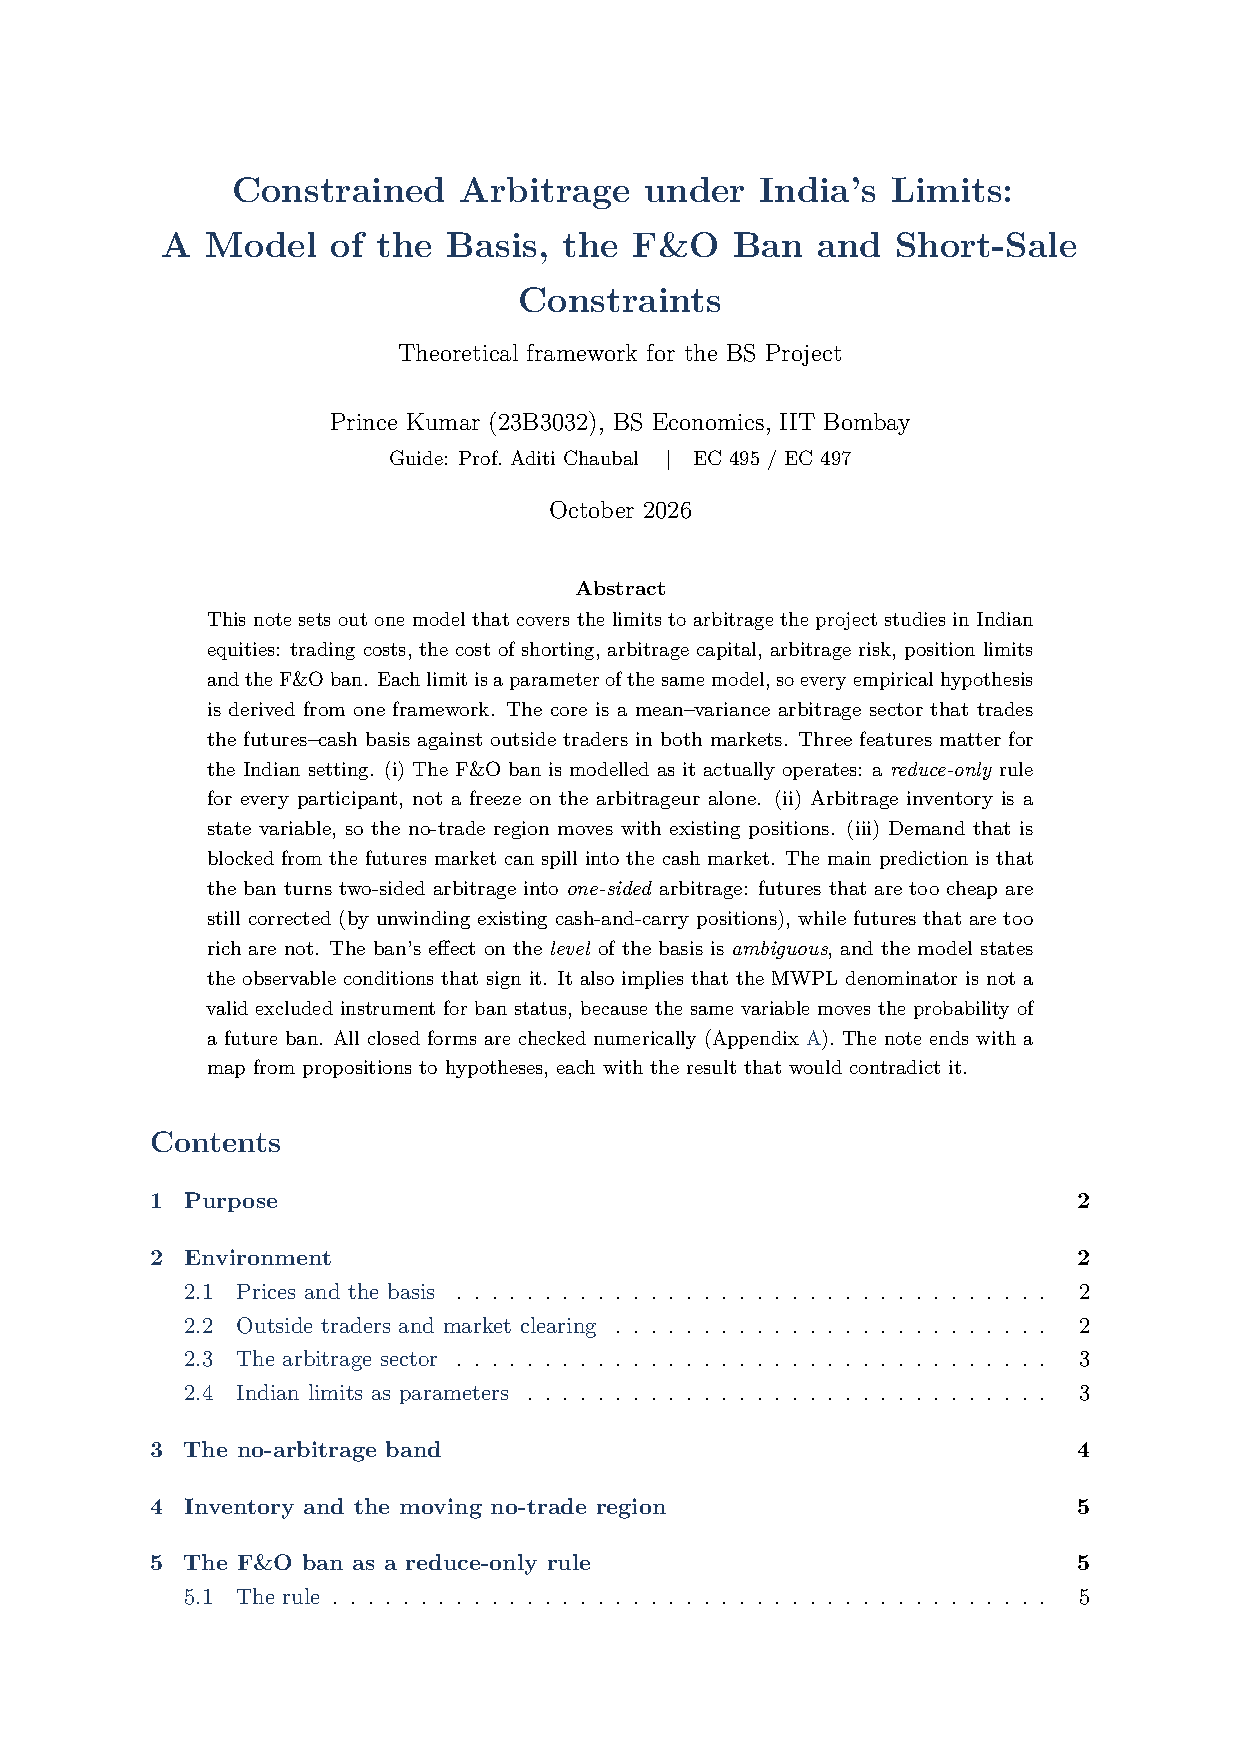
\includepdf[pages=-,pagecommand={\thispagestyle{empty}}]{../BSP_Model_C_Constrained_Arbitrage_India.pdf}

\chapter*{References}
\addcontentsline{toc}{chapter}{References}
\small
\begin{description}[leftmargin=1.2em,itemsep=1pt,font=\normalfont]
\item Aggarwal, N. (2015). Limits to arbitrage: The case of single stock futures and spot prices. IGIDR Working Paper WP-2015-010.
\item Amihud, Y. (2002). Illiquidity and stock returns: Cross-section and time-series effects. \emph{Journal of Financial Markets} 5(1), 31-56.
\item Bali, T., N. Cakici and R. Whitelaw (2011). Maxing out: Stocks as lotteries and the cross-section of expected returns. \emph{Journal of Financial Economics} 99(2), 427-446.
\item Brennan, M. and E. Schwartz (1990). Arbitrage in stock index futures. \emph{Journal of Business} 63(1), S7-S31.
\item Callaway, B. and P. Sant'Anna (2021). Difference-in-differences with multiple time periods. \emph{Journal of Econometrics} 225(2), 200-230.
\item Calonico, S., M. Cattaneo and R. Titiunik (2014). Robust nonparametric confidence intervals for regression-discontinuity designs. \emph{Econometrica} 82(6), 2295-2326.
\item Cattaneo, M., M. Jansson and X. Ma (2020). Simple local polynomial density estimators. \emph{Journal of the American Statistical Association} 115(531), 1449-1455.
\item Corwin, S. and P. Schultz (2012). A simple way to estimate bid-ask spreads from daily high and low prices. \emph{Journal of Finance} 67(2), 719-760.
\item Diamond, D. and R. Verrecchia (1987). Constraints on short-selling and asset price adjustment to private information. \emph{Journal of Financial Economics} 18(2), 277-311.
\item Dwyer, G., P. Locke and W. Yu (1996). Index arbitrage and nonlinear dynamics between the S\&P 500 futures and cash. \emph{Review of Financial Studies} 9(1), 301-332.
\item Gagnon, L. (2018). Short sale constraints and single stock futures introductions. \emph{Financial Review} 53(1), 5-50.
\item Gromb, D. and D. Vayanos (2010). Limits of arbitrage. \emph{Annual Review of Financial Economics} 2, 251-275.
\item Hou, K. and T. Moskowitz (2005). Market frictions, price delay, and the cross-section of expected returns. \emph{Review of Financial Studies} 18(3), 981-1020.
\item Kolari, J. and S. Pynn\"onen (2010). Event study testing with cross-sectional correlation of abnormal returns. \emph{Review of Financial Studies} 23(11), 3996-4025.
\item McCrary, J. (2008). Manipulation of the running variable in the regression discontinuity design: A density test. \emph{Journal of Econometrics} 142(2), 698-714.
\item Miller, E. (1977). Risk, uncertainty, and divergence of opinion. \emph{Journal of Finance} 32(4), 1151-1168.
\item Newey, W. and K. West (1987). A simple, positive semi-definite, heteroskedasticity and autocorrelation consistent covariance matrix. \emph{Econometrica} 55(3), 703-708.
\item Saurav, S., P. Srivastava and S. K. Agarwalla (2026). Decoupled: Disagreement, short-sale constraints, and law-of-one-price violations around earnings announcements. Working paper, SSRN.
\item Sehgal, S., V. Vasishth and F. Deisting (2024). Lottery factor and stock returns: Evidence from India. \emph{Borsa Istanbul Review} 24, 449-459.
\item Shankar, R. L., G. Sankar and K. Kiran Kumar (2019). Mispricing in single stock futures: Empirical examination of Indian markets. \emph{Emerging Markets Finance and Trade} 55(7), 1619-1633.
\item Shleifer, A. and R. Vishny (1997). The limits of arbitrage. \emph{Journal of Finance} 52(1), 35-55.
\item Stambaugh, R., J. Yu and Y. Yuan (2015). Arbitrage asymmetry and the idiosyncratic volatility puzzle. \emph{Journal of Finance} 70(5), 1903-1948.
\item Sun, L. and S. Abraham (2021). Estimating dynamic treatment effects in event studies with heterogeneous treatment effects. \emph{Journal of Econometrics} 225(2), 175-199.
\item Ters, K. and J. Urban (2020). Estimating unknown arbitrage costs: Evidence from a 3-regime threshold vector error correction model. \emph{Journal of Financial Markets} 47, 100503.
\item Tse, Y. (2001). Index arbitrage with heterogeneous investors: A smooth transition error-correction analysis. \emph{Journal of Banking and Finance} 25(10), 1829-1855.
\end{description}
\vspace{6pt}
{\sloppy\noindent\textbf{Regulatory documents.} SEBI circular MRD/DoP/SE/Dep/Cir-14/2007 (20 December 2007) and
SEBI/HO/MRD/MRD-PoD-3/P/CIR/2024/1 (5 January 2024), short selling; SEBI/DNPD/Cir-31/2006 (22 September 2006), MWPL; SEBI
press releases 18/2020 (20 March 2020) and 59/2020 (25 November 2020); SEBI/HO/MRD/MRD-PoD-2/P/CIR/2024/116 (30 August
2024), F\&O eligibility; SEBI/HO/MRD/TPD-1/P/CIR/2025/79 (29 May 2025), position limits and the ban rule; NSE Clearing
circular 119/2025 (8 September 2025) and its FAQ (13 October 2025); NSE circular 1/2018 on STT for physically settled
derivatives; NSE circulars FATAX56235 and FATAX73524 (STT from April 2023 and April 2026).\par}


\end{document}
